\documentclass{article}
\usepackage{amsthm}
\usepackage{amsmath}
\usepackage{graphicx}
\usepackage{multirow}
\usepackage{tikz}
\usepackage{wasysym}
\newtheorem{problem}{Problem}

\begin{document}
\title{Divide and Conquer}
\author{Henry Z. Lo}
\maketitle

\section{Divide and Conquer}
\subsection{Merge sort}
Recall the merge sort algorithm for sorting an integer array $x$:
\begin{enumerate}
\item Split $x$ into one element subarray.
\item Merge pairs of neighboring subarrays into a sorted subarray.  Weave together the smaller elements of both arrays first.
\item Continue step 2 until done.
\end{enumerate}

See Figure \ref{merge} for a visual.

\begin{figure}
\centering
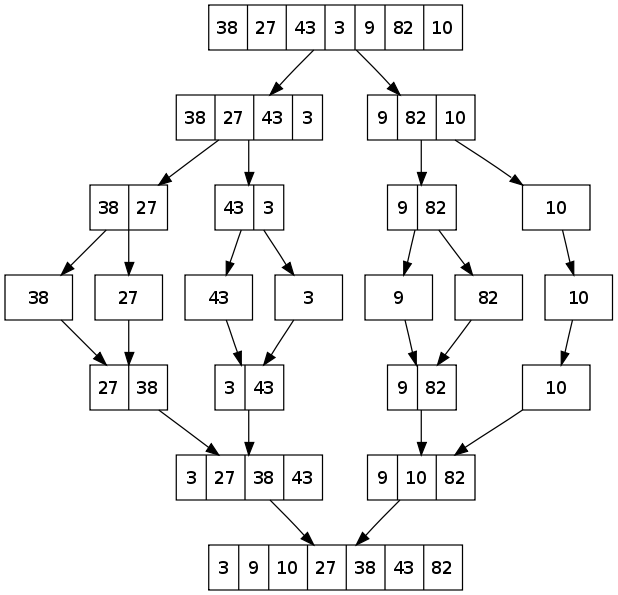
\includegraphics[width=\textwidth]{img/merge-sort.png}
\caption{Merge sort.\label{merge}}
\end{figure}

By the time the algorithm finishes, the array is sorted.  This scheme is efficient because there are merging sorted arrays can be done in linear time.  Since there are $\log n$ merges, this is an $O(n \log n)$  algorithm.

\subsection{Divide and conquer algorithms}
Divide and conquer algorithms can be broken down into three steps:
\begin{itemize}
\item Fracturing the problem into subproblems.
\item Solving subproblems recursively.
\item Combining these subproblems to arrive at the optimal solution.
\end{itemize}

Problems which can be solved by divide and conquer usually have the following properties:
\begin{itemize}
\item The smallest subproblems are trivial to solve.
\item Larger problems can be solved efficiently by combining solved subproblems.
\end{itemize}

Merge sort fits into this example.

\subsection{Binary search}
Given a sorted integer array, if we are looking for an integer $x$, we can throw away roughly half the remaining array with one comparison.  For example, if we are looking for 6 in the following array, this would be the series of viable candidates during binary search.
\begin{gather*}
\texttt{[1,5,6,8,10,13,14]} \\
\texttt{[1,5,6]} \\
\texttt{[6]}
\end{gather*}

This solution yields $O(\log n)$ comparisons.  This algorithm works because $x$ is in at most one half of the array; once we have deduced which part it's not in, we can disregard it.

Without question, this algorithm involves division.  It is arguable whether or not there is a "conquer" step.

\section{Other Examples}
\subsection{Quicksort}
Quicksort is another divide and conquer sorting algorithm, similar to mergesort.  However, the sorting is done during the divide step, and the combined result is the sorted array.

The algorithm:
\begin{enumerate}
\item Pick an element $x$ from the array.
\item Put everything less than $x$ to the left of $x$, and everything greater or equal to its right.
\item Repeat the second step, until we get to trivially sorted arrays.
\item Combine pairs of subarrays until we get the sorted array.
\end{enumerate}

Even though it is $O(n^2)$ in the worst case (if we keep splitting off one element at a time), on average it is $O(n \log n)$.

\subsection{Closest pair of points}
Consider a set of points $\{(x_1,y_1),(x_2,y_2),\ldots,(x_n,y_n)\}$.  We want to find the closest pair of points.  See Figure \ref{points}.

\begin{figure}
\centering
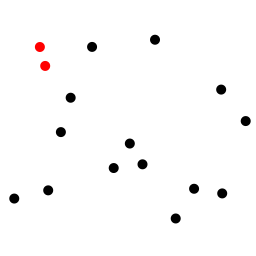
\includegraphics[width=0.4\textwidth]{img/points.png}
\caption{Closest pair of points.\label{pair}}
\end{figure}

We can do this with a similar algorithm with merge sort:

\begin{enumerate}
\item Sort all points by $x$ values.
\item Divide:
\begin{enumerate}
\item Find the point on the $x$ axis where half the points are on the left, and half on the right.
\item Split into two subarrays.
\item Repeat steps 2 and 3 until we get to subarrays with two points.
\end{enumerate}
\item Calculate nearest pair for each subarray.
\item Combine:
\begin{enumerate}
\item Return the new nearest pair.  This is either one of the two subarray pairs, or a new pair with points in different subarrays.
\end{enumerate}
\end{enumerate}

We need to find the nearest pair between subarrays to compare with the two nearest subarray pairs.  Let the smaller distance of the nearest subarray pairs be $d$.  If there is a pair of points in different subarrays which is closer than $d$, then that is the pair we want.

See Figure \ref{closest-pair} for a visual.  Let $p_1$ and $p_2$ be those two points.  $p_2$ must be within a $d \times 2d$ rectangle of $p_1$, and on the opposite side of the line.  There are a limited number of possible points on the opposite side, because they must be at least $d$ apart.

\begin{figure}
\centering
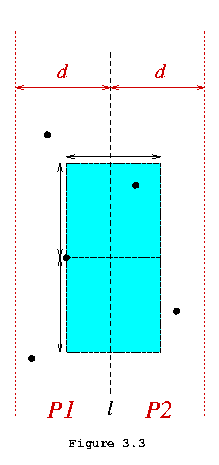
\includegraphics[width=0.3\textwidth]{img/closest-pair.png}
\caption{Closest pair of points problem, when points are in different subarrays.\label{closest-pair}}
\end{figure}

\subsection{Convex hull}
The convex hull of a set of points is a subset which contains all the others.  You can think of it as the set of points a rubber band would touch.  See Figure \ref{hull}.

\begin{figure}
\centering
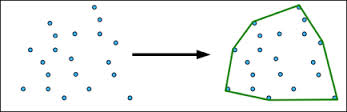
\includegraphics[width=0.8\textwidth]{img/convex-hull.jpg}
\caption{Convex hull.\label{hull}}
\end{figure}

There are many methods to finding convex hulls.  We can use divide and conquer, if we divide just as we did in the closest pairs problem.  Given two sets of points, their convex hulls can be combined to form the convex hull of the two sets combined.

However, we need to compute the upper and lower \textit{tangents} that connect the two convex hulls (see Figure \ref{combine-hulls}), and throw out all the points in between.

\begin{figure}
\centering
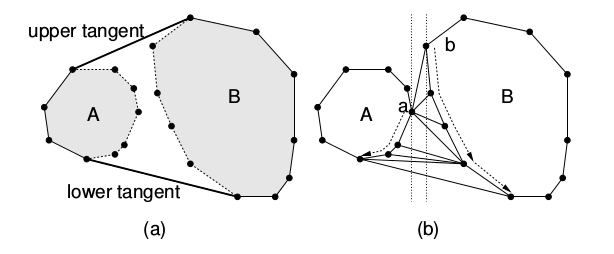
\includegraphics[width=0.8\textwidth]{img/combine_hull.png}
\caption{Combining convex hulls.\label{combine-hull}}
\end{figure}

We can do this using the following iterative procedure for the bottom tangent:
\begin{enumerate}
\item Start at the leftmost point ($a$) on the left set of points, and the rightmost point ($b$) on the right set.
\item If some point on the left convex hull is below the line $ab$, then select the next counterclockwise point to be the new $a$.
\item Likewise for $b$, but update clockwise.
\end{enumerate}
Once the procedure is done, then $ab$ is the lower tangent.  This is a linear time procedure.



\end{document}
